\documentclass[conference]{IEEEtran}
\IEEEoverridecommandlockouts
% The preceding line is only needed to identify funding in the first footnote. If that is unneeded, please comment it out.
\usepackage{cite}
\usepackage{amsmath,amssymb,amsfonts}
\usepackage{algorithmic}
\usepackage{graphicx}
\usepackage{textcomp}
\usepackage{xcolor}
\usepackage{multirow}
\def\BibTeX{{\rm B\kern-.05em{\sc i\kern-.025em b}\kern-.08em
    T\kern-.1667em\lower.7ex\hbox{E}\kern-.125emX}}
\begin{document}

\title{UNAT: An Unstructured Accelerated Toolkit based on Sunway architecture\\
\thanks{Identify applicable funding agency here. If none, delete this.}
}

\author{\IEEEauthorblockN{1\textsuperscript{st} Hongbin Liu}
\IEEEauthorblockA{\textit{National Supercomputing Center} \\ \textit{in Wuxi}\\
Wuxi, China \\
lhb8125@gmail.com}
\and
\IEEEauthorblockN{2\textsuperscript{nd} Hu Ren}
\IEEEauthorblockA{\textit{National Supercomputing Center} \\ \textit{in Wuxi}\\
Wuxi, China \\
email address}
\and 
\IEEEauthorblockN{3\textsuperscript{rd} Hanfeng Gu}
\IEEEauthorblockA{\textit{Tsinghua University}\\
\textit{National Supercomputing Center} \\ \textit{in Wuxi}\\
Wuxi, China \\
email address}
\and
\IEEEauthorblockN{4\textsuperscript{rd} Fei Gao}
\IEEEauthorblockA{
\textit{National Supercomputing Center} \\ \textit{in Wuxi}\\
Wuxi, China \\
email address}
\and
\IEEEauthorblockN{5\textsuperscript{th} Wei Xue}
\IEEEauthorblockA{\textit{Tsinghua University}\\
\textit{National Supercomputing Center} \\ \textit{in Wuxi}\\
Wuxi, China \\
email address}
\and
\IEEEauthorblockN{6\textsuperscript{th} Guangwen Yang}
\IEEEauthorblockA{\textit{Tsinghua University}\\
\textit{National Supercomputing Center} \\ \textit{in Wuxi}\\
Wuxi, China \\
email address}
}

\maketitle

\begin{abstract}
This document is a model and instructions for \LaTeX.
This and the IEEEtran.cls file define the components of your paper [title, text, heads, etc.]. *CRITICAL: Do Not Use Symbols, Special Characters, Footnotes, 
or Math in Paper Title or Abstract.
\end{abstract}

\begin{IEEEkeywords}
component, formatting, style, styling, insert
\end{IEEEkeywords}

\section{Introduction}
This document is a model and instructions for \LaTeX.
Please observe the conference page limits. 

\section{Ease of Use}

\subsection{Maintaining the Integrity of the Specifications}

The IEEEtran class file is used to format your paper and style the text. All margins, 
column widths, line spaces, and text fonts are prescribed; please do not 
alter them. You may note peculiarities. For example, the head margin
measures proportionately more than is customary. This measurement 
and others are deliberate, using specifications that anticipate your paper 
as one part of the entire proceedings, and not as an independent document. 
Please do not revise any of the current designations.

\section{Prepare Your Paper Before Styling}
Before you begin to format your paper, first write and save the content as a 
separate text file. Complete all content and organizational editing before 
formatting. Please note sections \ref{AA}--\ref{SCM} below for more information on 
proofreading, spelling and grammar.

Keep your text and graphic files separate until after the text has been 
formatted and styled. Do not number text heads---{\LaTeX} will do that 
for you.

\subsection{Abbreviations and Acronyms}\label{AA}
Define abbreviations and acronyms the first time they are used in the text, 
even after they have been defined in the abstract. Abbreviations such as 
IEEE, SI, MKS, CGS, ac, dc, and rms do not have to be defined. Do not use 
abbreviations in the title or heads unless they are unavoidable.

\subsection{Units}
\begin{itemize}
\item Use either SI (MKS) or CGS as primary units. (SI units are encouraged.) English units may be used as secondary units (in parentheses). An exception would be the use of English units as identifiers in trade, such as ``3.5-inch disk drive''.
\item Avoid combining SI and CGS units, such as current in amperes and magnetic field in oersteds. This often leads to confusion because equations do not balance dimensionally. If you must use mixed units, clearly state the units for each quantity that you use in an equation.
\item Do not mix complete spellings and abbreviations of units: ``Wb/m\textsuperscript{2}'' or ``webers per square meter'', not ``webers/m\textsuperscript{2}''. Spell out units when they appear in text: ``. . . a few henries'', not ``. . . a few H''.
\item Use a zero before decimal points: ``0.25'', not ``.25''. Use ``cm\textsuperscript{3}'', not ``cc''.)
\end{itemize}

\subsection{Equations}
Number equations consecutively. To make your 
equations more compact, you may use the solidus (~/~), the exp function, or 
appropriate exponents. Italicize Roman symbols for quantities and variables, 
but not Greek symbols. Use a long dash rather than a hyphen for a minus 
sign. Punctuate equations with commas or periods when they are part of a 
sentence, as in:
\begin{equation}
a+b=\gamma\label{eq}
\end{equation}

Be sure that the 
symbols in your equation have been defined before or immediately following 
the equation. Use ``\eqref{eq}'', not ``Eq.~\eqref{eq}'' or ``equation \eqref{eq}'', except at 
the beginning of a sentence: ``Equation \eqref{eq} is . . .''

\subsection{\LaTeX-Specific Advice}

Please use ``soft'' (e.g., \verb|\eqref{Eq}|) cross references instead
of ``hard'' references (e.g., \verb|(1)|). That will make it possible
to combine sections, add equations, or change the order of figures or
citations without having to go through the file line by line.

Please don't use the \verb|{eqnarray}| equation environment. Use
\verb|{align}| or \verb|{IEEEeqnarray}| instead. The \verb|{eqnarray}|
environment leaves unsightly spaces around relation symbols.

Please note that the \verb|{subequations}| environment in {\LaTeX}
will increment the main equation counter even when there are no
equation numbers displayed. If you forget that, you might write an
article in which the equation numbers skip from (17) to (20), causing
the copy editors to wonder if you've discovered a new method of
counting.

{\BibTeX} does not work by magic. It doesn't get the bibliographic
data from thin air but from .bib files. If you use {\BibTeX} to produce a
bibliography you must send the .bib files. 

{\LaTeX} can't read your mind. If you assign the same label to a
subsubsection and a table, you might find that Table I has been cross
referenced as Table IV-B3. 

{\LaTeX} does not have precognitive abilities. If you put a
\verb|\label| command before the command that updates the counter it's
supposed to be using, the label will pick up the last counter to be
cross referenced instead. In particular, a \verb|\label| command
should not go before the caption of a figure or a table.

Do not use \verb|\nonumber| inside the \verb|{array}| environment. It
will not stop equation numbers inside \verb|{array}| (there won't be
any anyway) and it might stop a wanted equation number in the
surrounding equation.

\subsection{Some Common Mistakes}\label{SCM}
\begin{itemize}
\item The word ``data'' is plural, not singular.
\item The subscript for the permeability of vacuum $\mu_{0}$, and other common scientific constants, is zero with subscript formatting, not a lowercase letter ``o''.
\item In American English, commas, semicolons, periods, question and exclamation marks are located within quotation marks only when a complete thought or name is cited, such as a title or full quotation. When quotation marks are used, instead of a bold or italic typeface, to highlight a word or phrase, punctuation should appear outside of the quotation marks. A parenthetical phrase or statement at the end of a sentence is punctuated outside of the closing parenthesis (like this). (A parenthetical sentence is punctuated within the parentheses.)
\item A graph within a graph is an ``inset'', not an ``insert''. The word alternatively is preferred to the word ``alternately'' (unless you really mean something that alternates).
\item Do not use the word ``essentially'' to mean ``approximately'' or ``effectively''.
\item In your paper title, if the words ``that uses'' can accurately replace the word ``using'', capitalize the ``u''; if not, keep using lower-cased.
\item Be aware of the different meanings of the homophones ``affect'' and ``effect'', ``complement'' and ``compliment'', ``discreet'' and ``discrete'', ``principal'' and ``principle''.
\item Do not confuse ``imply'' and ``infer''.
\item The prefix ``non'' is not a word; it should be joined to the word it modifies, usually without a hyphen.
\item There is no period after the ``et'' in the Latin abbreviation ``et al.''.
\item The abbreviation ``i.e.'' means ``that is'', and the abbreviation ``e.g.'' means ``for example''.
\end{itemize}
An excellent style manual for science writers is \cite{b7}.

\subsection{Authors and Affiliations}
\textbf{The class file is designed for, but not limited to, six authors.} A 
minimum of one author is required for all conference articles. Author names 
should be listed starting from left to right and then moving down to the 
next line. This is the author sequence that will be used in future citations 
and by indexing services. Names should not be listed in columns nor group by 
affiliation. Please keep your affiliations as succinct as possible (for 
example, do not differentiate among departments of the same organization).

\subsection{Identify the Headings}
Headings, or heads, are organizational devices that guide the reader through 
your paper. There are two types: component heads and text heads.

Component heads identify the different components of your paper and are not 
topically subordinate to each other. Examples include Acknowledgments and 
References and, for these, the correct style to use is ``Heading 5''. Use 
``figure caption'' for your Figure captions, and ``table head'' for your 
table title. Run-in heads, such as ``Abstract'', will require you to apply a 
style (in this case, italic) in addition to the style provided by the drop 
down menu to differentiate the head from the text.

Text heads organize the topics on a relational, hierarchical basis. For 
example, the paper title is the primary text head because all subsequent 
material relates and elaborates on this one topic. If there are two or more 
sub-topics, the next level head (uppercase Roman numerals) should be used 
and, conversely, if there are not at least two sub-topics, then no subheads 
should be introduced.

\subsection{Figures and Tables}
\paragraph{Positioning Figures and Tables} Place figures and tables at the top and 
bottom of columns. Avoid placing them in the middle of columns. Large 
figures and tables may span across both columns. Figure captions should be 
below the figures; table heads should appear above the tables. Insert 
figures and tables after they are cited in the text. Use the abbreviation 
``Fig.~\ref{fig}'', even at the beginning of a sentence.

\begin{table}[htbp]
\caption{Table Type Styles}
\begin{center}
\begin{tabular}{|c|c|c|c|}
\hline
\textbf{Table}&\multicolumn{3}{|c|}{\textbf{Table Column Head}} \\
\cline{2-4} 
\textbf{Head} & \textbf{\textit{Table column subhead}}& \textbf{\textit{Subhead}}& \textbf{\textit{Subhead}} \\
\hline
copy& More table copy$^{\mathrm{a}}$& &  \\
\hline
\multicolumn{4}{l}{$^{\mathrm{a}}$Sample of a Table footnote.}
\end{tabular}
\label{tab1}
\end{center}
\end{table}

\begin{figure}[htbp]
\centerline{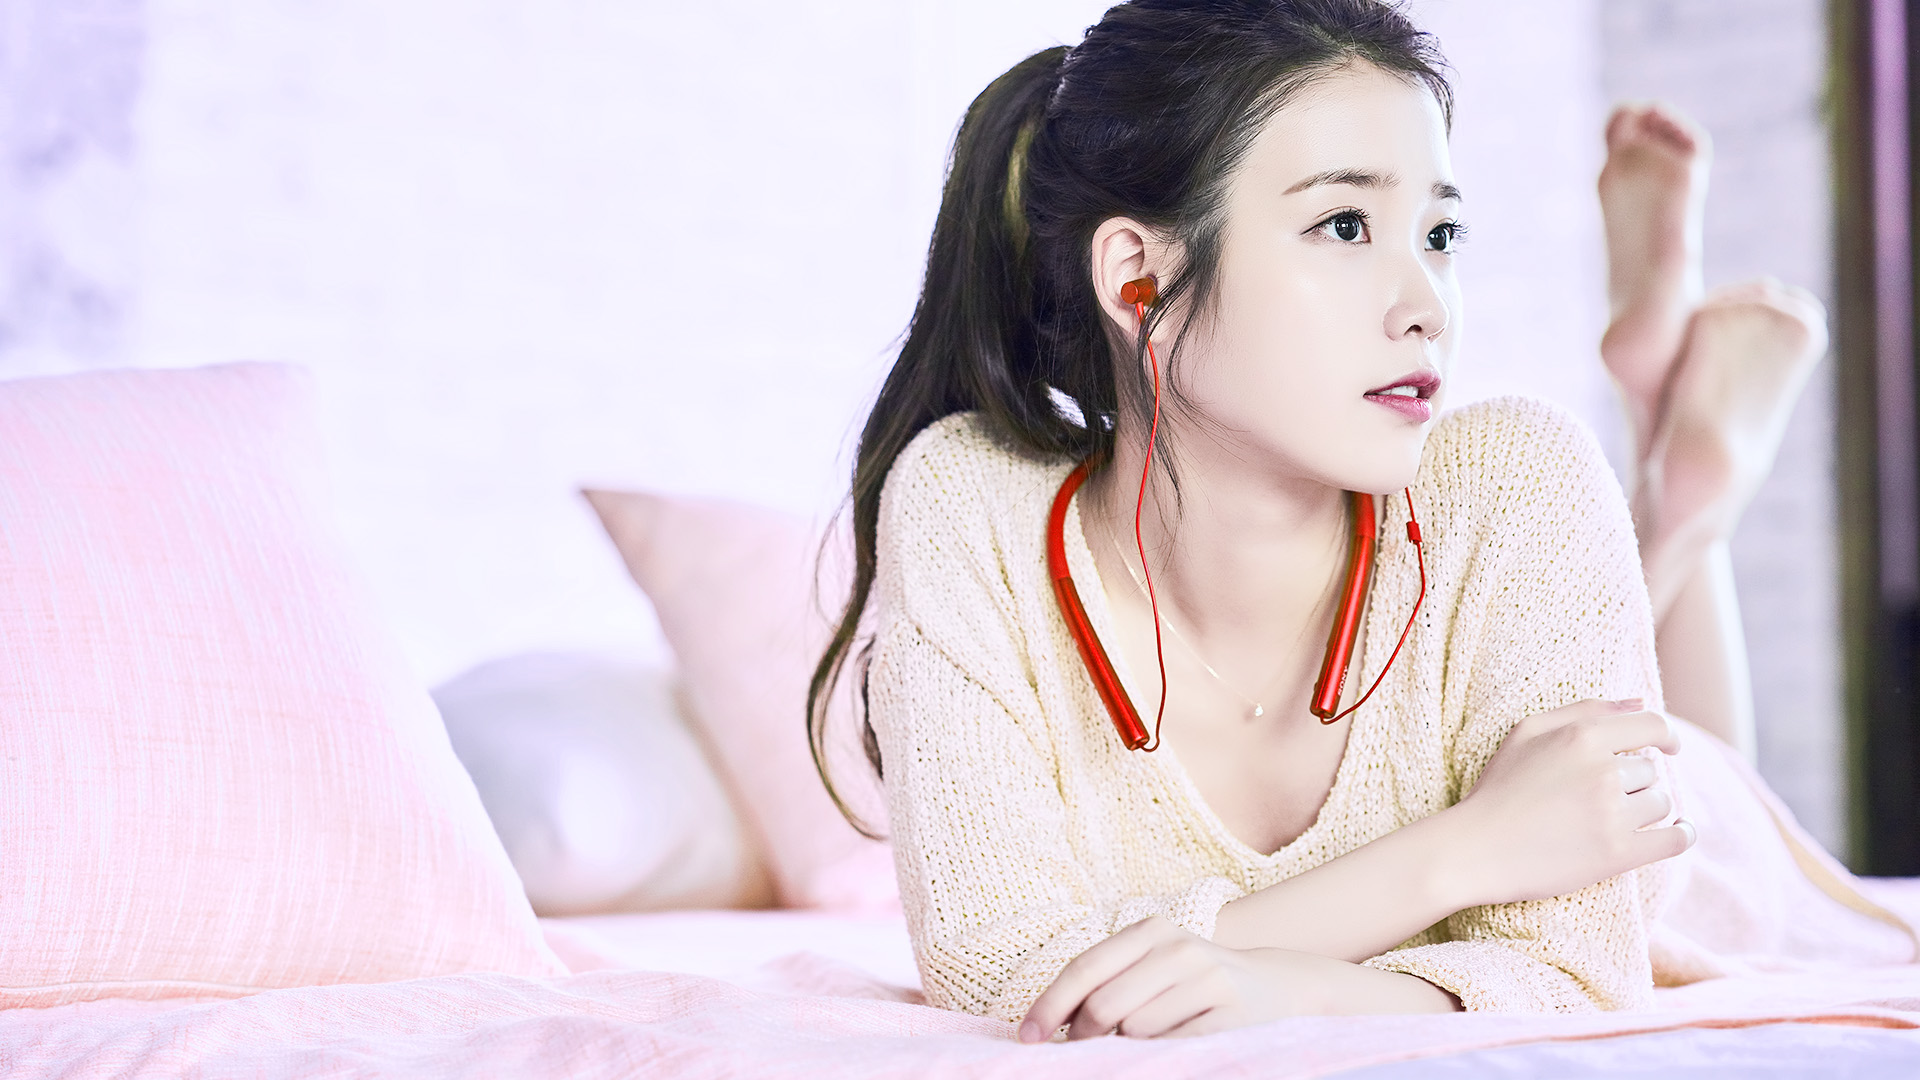
\includegraphics[width=0.45\textwidth]{fig1.jpg}}
\caption{Example of a figure caption.}
\label{fig}
\end{figure}


Figure Labels: Use 8 point Times New Roman for Figure labels. Use words 
rather than symbols or abbreviations when writing Figure axis labels to 
avoid confusing the reader. As an example, write the quantity 
``Magnetization'', or ``Magnetization, M'', not just ``M''. If including 
units in the label, present them within parentheses. Do not label axes only 
with units. In the example, write ``Magnetization (A/m)'' or ``Magnetization 
\{A[m(1)]\}'', not just ``A/m''. Do not label axes with a ratio of 
quantities and units. For example, write ``Temperature (K)'', not 
``Temperature/K''.

\section{Design and API}

\section{Parallelization Strategy}

\subsection{SW26010 Many-core processor}

The SW26010 many-core processor is the basic component unit of the Sunway TaihuLight supercomputer, which is designed by Shanghai High Performance IC Design Center. The detail of Sunway architecture is illustrated in Fig. \ref{sw26010}.
\begin{figure}[tbp]
\centerline{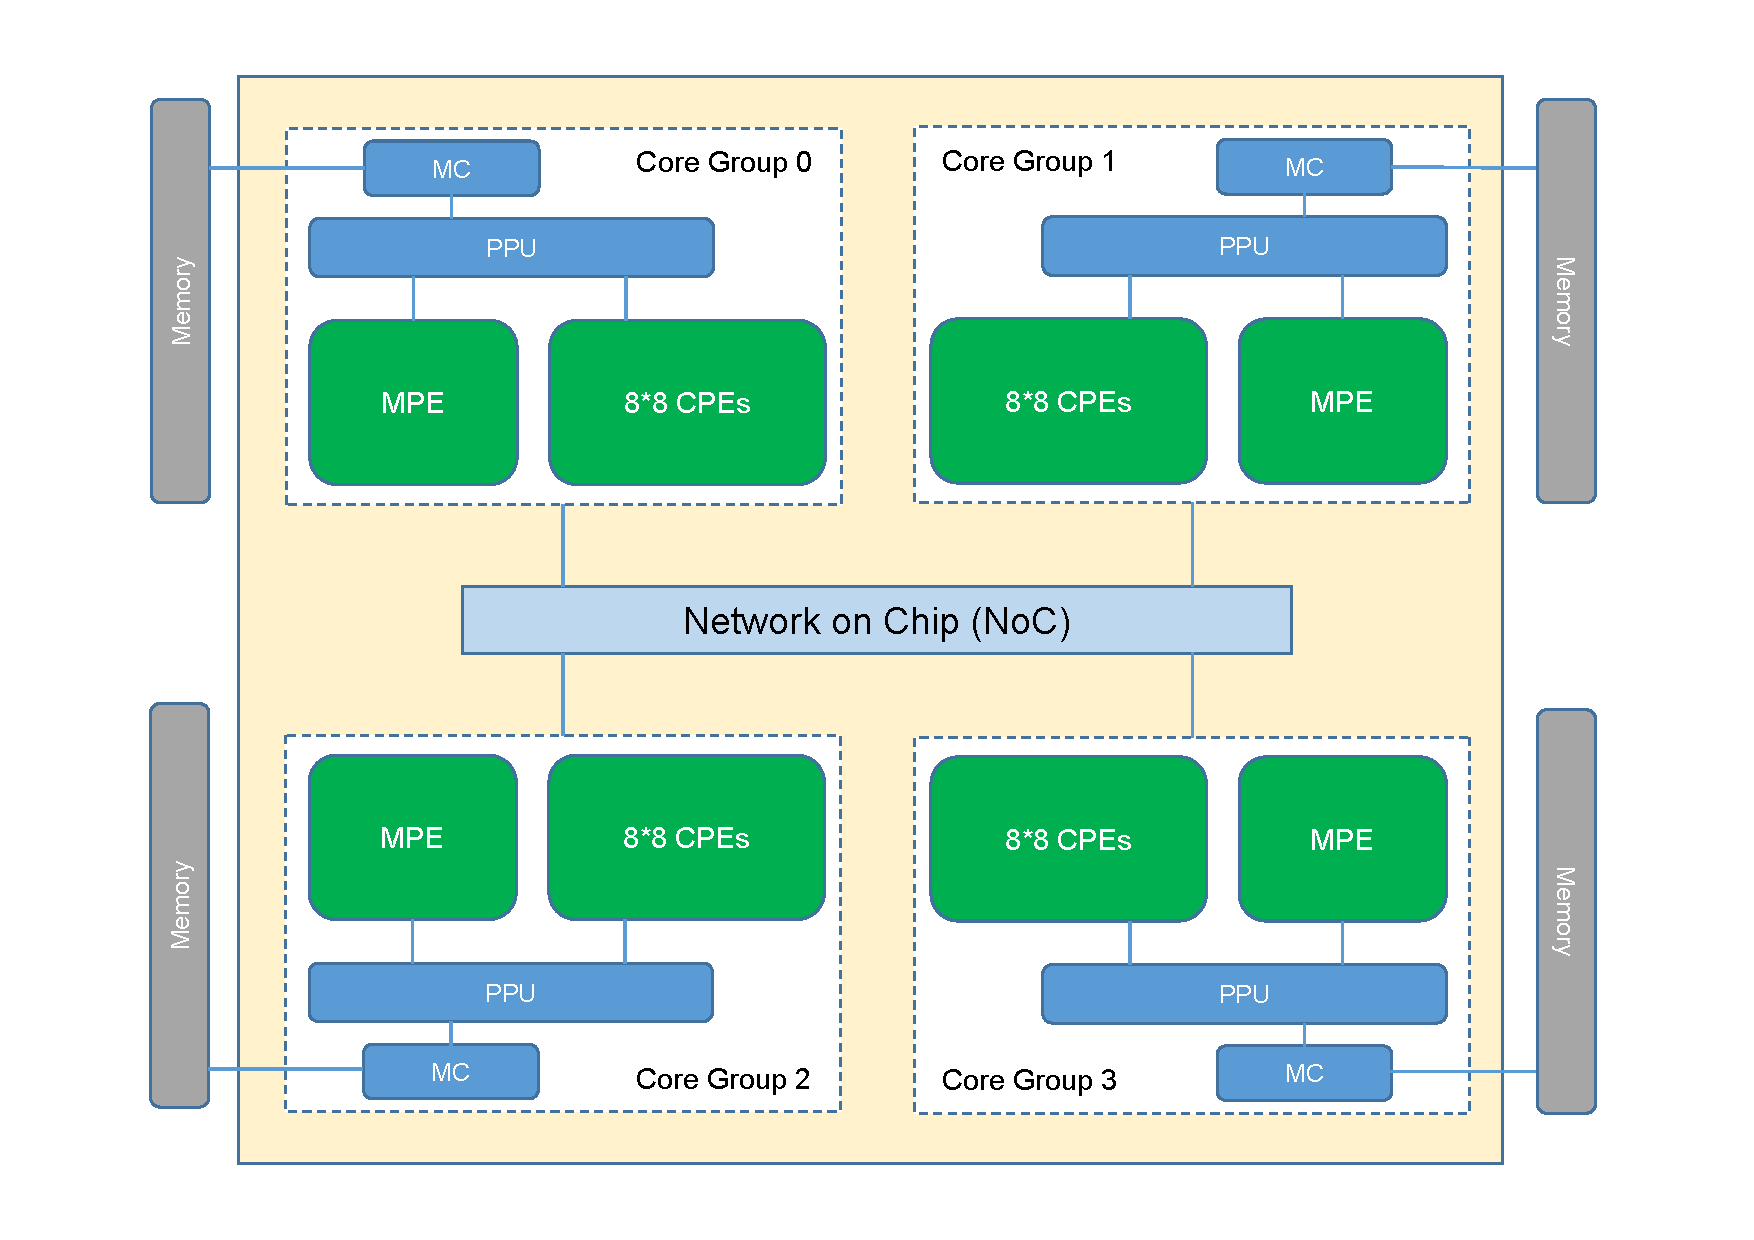
\includegraphics[width=0.49\textwidth]{sw26010.pdf}}
\caption{The architecture of Sunway processor}
\label{sw26010}
\end{figure}
It can provide a peak performance of 3.06 TFlops and a performance-to-power ratio of 10 GFlops/Watt. The processor contains four Core Groups (CGs) and each CG is composed of one Management Processing Element (MPE), one DDR3 Memory Controller (MC) and one Computing Processing Elements (CPEs) cluster with 64 CPEs organized as 8 by 8 mesh. Each CG has 765 GFlops double-precision peak performance and 34.1 GB/s theoretical memory bandwidth. The MPE targeting at task management is a complete 64-bit RISC core with a frequency of 1.45 GHz, supporting complete interrupt functions and out-of-order execution. In contrast, CPE is a simplified 64-bit RISC core to maximize the aggregated computing power.

As for the memory hierarchy, each CG connects to its own 8GB DDR3 memory through MC, accessed through Direct Memory Access (DMA) for the MPE and CPEs. The Network on Chip manage the memory of four CGs and the size of each CG's private memory space can be customized by users. The MPE has a 32KB L1 instruction cache, a 32KB L1 data cache and a 256KB L2 cache for both instrcution and data, while each CPE provides a 16KB instruction cache and a 64KB Local Device Memory (LDM). The programmable LDM is controlled by users through software. The processor provides an important data sharing capability across the CPEs: register communication, which enables the CPEs in the same row or column can communicate with each other with ten clock cycles. A performance model based on the three-level (REG-LDM-MEM) memory hierarchy was proposed \cite{b16}.

\subsection{Performance challenges for mapping UNAT to SW26010}

% this section should be included in chapter: Design and API.
%Different from the stencils on structured mesh, the data structure of unstructured topology is commonly described as an adjacency graph or sparse matrix. Take the finite volume dicretization method as example, the topology can be represented as a symmetric sparse matrix in different formats such as Compressed Coordinate (COO), Compressed Sparse Row (CSR) and Lower-Diagonal-Upper (LDU). LDU is a more index-saving matrix format, in which a topology-symmetric matrix can be store with half coordinates of COO. CSR and LDU format are supported in UNAT.

Different from the stencils on structured mesh, the data structure of unstructured topology is commonly described as an adjacency graph or sparse matrix. Generally, this kind of computation introduces two main performance challenges on many-core processors: low arithmetic density and irregular memory access.

Although high order numerical schemes such as Discontinuous-Galekin (DG) method are also well adopted in some solvers, numerical schemes with orders no more than 2 are most frequently configured to guarantee the stability and convergence in complex geometry simulation in finite volume method. Taking several representative operators widely used in OpenFOAM as example, the ratio of float operations to the number of DMA is only 1 and 2 for integration and interpolation respectively. Considering the high ratio of Flops to bandwidth of SW26010 theoretically, this kind of computation becomes strong memory bandwidth limited.

According to the computation nature of unstructured mesh, the data access pattern to memory is indirect and irregular. As measured in real case, the bandwidth (the largest distance from the coefficients to the diagonal) reach up to 7K for an topology matrix with 120K cells even with minimizing reordering. The irregular memory access will increase cache miss and unnecessary memory access times. This problem may be alleviated on platform with larger cache size such as 10MB $3_{rd}$ level cache on Intel multi-core processor or large memory bandwidth such as NVIDIA Tesla K80 (480GB/s). While for SW26010 processor, the bandwidth is relatively low and one can not yield high performance with the default communication through DMA on the Sunway architecture. 

Register communication and LDM are provided for programmers as an efficient interface on Sunway architecture. However, we may suffer from significant performance degradation without careful data management. Therefore, we need to design an memory access and communication scheme to alleviate the memory bandwidth constrains.

\subsection{Multi-Level Block (MLB) method}

As mentioned above, the computational capability in unstructured mesh is limited extremely by the indirect and irregular addressing. Therefore, we propose Multi-Level Block (MLB) method and design a MPE-CPEs asynchronous parallel algorithm. Fig. \ref{mlb(overview)} presents the decomposition of an unstructured mesh and its matrix form with LDU format.
\begin{figure}[tbp]
\centerline{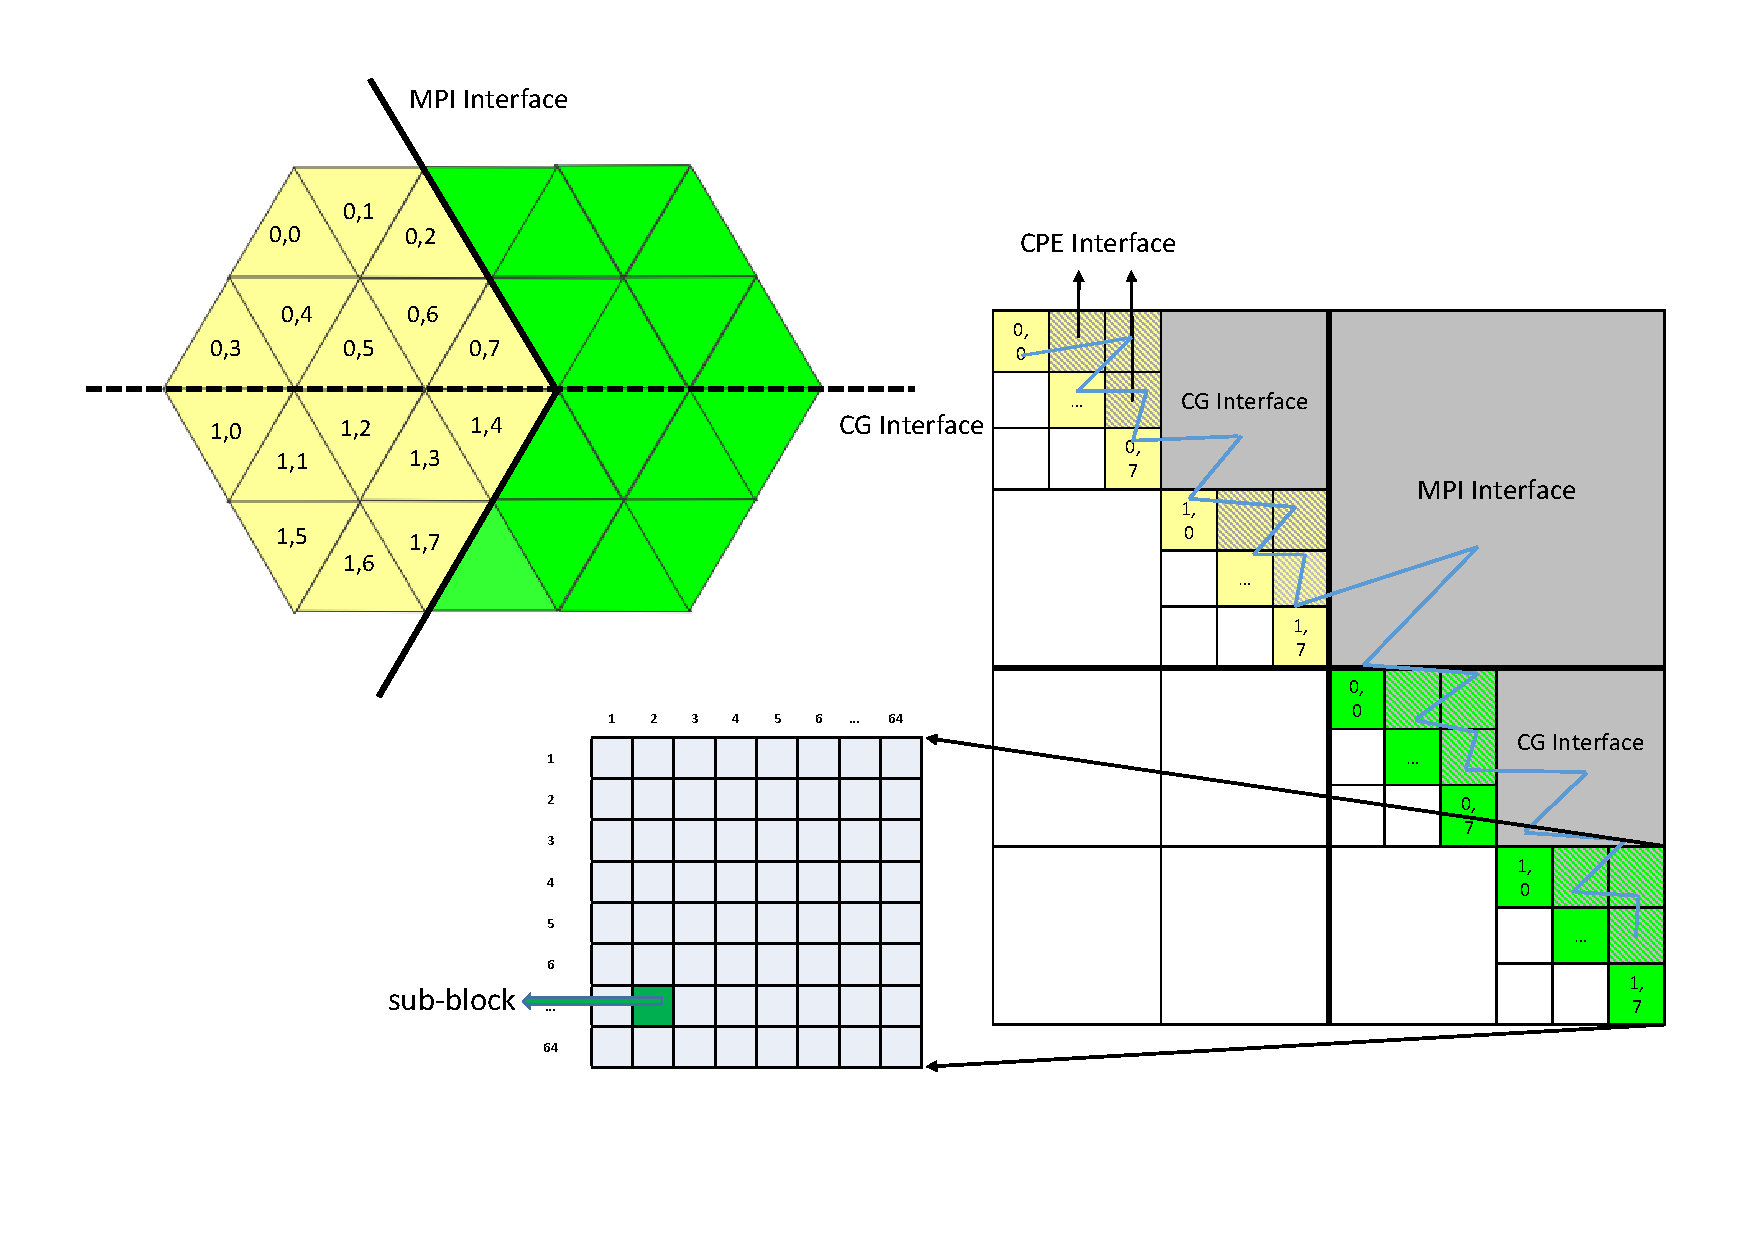
\includegraphics[width=0.49\textwidth]{mlb(overview).pdf}}
\caption{Multi-Level Block of unstructured mesh. The unstructured mesh is decomposed and assigned to two process, colored with yellow and green respectively. Three levels are connected by three interfaces: MPI interface, CG interface and CPEs interface.}
\label{mlb(overview)}
\end{figure}
The data structure in MLB is a non-uniform multi-block structure. The coarsest block (coarse-block) represents the mesh decomposition at MPI level. The non-zeros on coarse-blocks represent the internal faces of mesh cells inside one process assigned to a single CG, and the off-diagonal coarse-block is the MPI interface distributed on different processes. The medium block (block) is partitioned because of the limitation of LDM size and then the whole relevant data of blocks can be stored in LDM thoroughly. At this level, all blocks are categorized as internal blocks (marked as colored cells in the diagonal blocks) and CG interface blocks (marked as gray cells in the off-diagonal blocks), assigned to CPEs and MPE respectively with the data density into consideration. This pattern will introduce an read-write conflict between MPE and CPE if they are in charge of the same row. The issue can be eliminated through adding a bias to the row index of blocks in MPE relative to CPEs.

Finally, the finest block (sub-block) is decomposed based on the hardware of CG. The number of sub-block is set to a fixed value, 64, corresponding to the amount of CPEs of CG. The diagonal sub-block is "local" for the corresponding CPE and the off-diagonal sub-block is the CPE interface. The "local" data are loaded into LDM by DMA directly while the data in the interface are transferred by on-chip register communication because of the discreteness and sparsity. The blue filling curve in Fig. \ref{mlb(overview)} indicates the storage sequence of different blocks in memory. Generally, the priority rule is that the finer level block is prior to coarser ones and row block is prior to column block in the same level. Inside the sub-blocks, the face sequence is arbitrary. Taking advantage of the graph partition tool Metis, most face can be gathered in diagonal blocks for each level and interfaces can be minimized to a certain extent with load balance into consideration. So far we obtain an block-structured and organized data structure through MLB.

As for the computation of diagonal block in CPEs, one CPE is in charge of the sub-blocks in the same row. To explain the computational pattern of CPEs, we take the Sparse Matrix-Vector multiply (SpMV) as example. The coefficient matrix $A$ with LDU format is stored as three arrays, $lower$, $upper$ and $diag$ .

\subsubsection{test}

\section{Performance}

\subsection{Experiment Setup}
In this section, quantitative experiment results are presented discussed to evaluate the performance of UNAT. Sparse Matrix-vector Multiply (SpMV) is selected as the measured operator. It plays an important role in linear algebra algorithms, which is well adopted for computational fluid dynamic (CFD), molecular dynamics (MD), and some machine learning algorithm such as convolution neural network (CNN) deeply relies on SpMV. However, SpMV is not friendly for many-core architectures because of the irregular memory access and write conflicts \cite{b8} and then is appropriate to examine the efficiency of UNAT. As is mentioned above, we separate the specification of a computational operator with its parallel iteration details. Hence the specification of SpMV in UNAT is roughly identical to its implementation in the serial edition as is shown in \ref{spmvOps}. The UNAT API \textbf{define\_ops}, \textbf{accessArray}, \textbf{getArraySize} and \textbf{getArrayDims} are designed to define the operator and access the struct \textbf{Array} respectively. Two points need to be explained to improve the comprehensibility of UNAT API. Firstly, we introduce the dimensions \textbf{dims} in the loop in support of the AOS data storage pattern and the \textbf{dims} indicates the number of component in the struct; Secondly, we separate the computation of lower triangle from the upper triangle for the compatibility of LDU and CSR format, and then in CSR format, the computation of lower triangle is nonexistent and ignored. Therefore, the uniform and compatible operator can be defined to support different storage pattern and matrix format.

We perform various experiments to reveal the performance of UNAT thoroughly and the details are shown in \ref{expDetail}. MLB and RSS iterator mentioned above are the main performance object of UNAT and we will illustrate the results in the next sections respectively. We select two types of matrices, which are tested with two representative sparse matrices format, LDU and CSR. The matrix applied to MLB iterator is the boxTube16 case from the tutorials of OpenFOAM, which performs DNS with the finite volume scheme. The other one applied to RSS iterator is from the University of Florida Sparse Matrix Collection \cite{b9}, and it is used to solve Navier-Stokes and similar transport equations with finite element discretization. Both of them have series of matrices with similar topology and different non-zeros, ranging from 30K to 700K. Moreover, to compare to performance of UNAT across SOA and AOS storage pattern, we set four different numbers of components in struct and the values are corresponding to the variable types scalar, vector, symmetric matrix and unsymmetric matrix respectively. The storage pattern naturally transforms from AOS to SOA when the number of components equals to 1.

Our experiments are conducted on a CG of a Sunway SW26010 processor. The performance of SpMV on a CG because scientific applications on Sunway TaihuLight will generally adopt two-level parallelism and perform the computation problem, such as SpMV, within CG. The compiler flags are shown in \ref{flags}. \textbf{sw5cc} and \textbf{mpiCC} are the native compilers on Sunway and the \textbf{-OPT:IEEE\_arithmetic=2} flag is added to avoid the float exception situation. We use the application on MPE as our baseline for the performance comparison. All experiments are performed for five times and report the average results in double-precision floating-point arithmetic.


\begin{table}[]
\caption{The specification of SPMV operator in UNAT}
\begin{tabular}{l}
\hline Algorithm: SpMV operator                                                                                                                                                                                                                                                                                                                                                                                                                                                                                                                                                                                                                                                                                                                                                                                                                                                                                                                                                                                                                                                                                                                                                                                                                                                                                                                                                                                          \\ \hline
\begin{tabular}[c]{@{}l@{}}// define the SpMV wrapper interface\\ define\_ops(SpMV)\\ \{\\ \qquad swFloat *diag  = accessArray(selfConnData, 0);\\ \qquad swFloat *x     = accessArray(vertexData, 0);\\ \qquad swFloat *b     = accessArray(vertexData, 0);\\ \qquad swFloat *upper = accessArray(frontEdgeData, 0);\\ \qquad swFloat *lower = accessArray(backEdgeData, 0);\\         \\ \qquad swInt ivertex, iedge, idim;\\ \qquad swInt vertexNum = getArraySize(selfConnData);\\ \qquad dims = getArrayDims(selfConnData, 0);\\ \qquad for(ivertex=0;ivertex\textless{}vertexNum;ivertex++)\\ \qquad \{\\ \qquad \qquad for(idim=0;idim\textless{}dims;idim++)\\ \qquad \qquad \{\\ \qquad \qquad \qquad b{[}ivertex*dims+idim{]} \\ \qquad \qquad \qquad \qquad = diag{[}ivertex*dims+idim{]}*x{[}ivertex*dims+idim{]};\\ \qquad \qquad \}\\ \qquad \}\\ \\ \qquad dims = getArrayDims(frontEdgeData, 0);\\ \qquad swInt edgeNum = getArraySize(frontEdgeData);\\ \qquad for(iedge=0;iedge\textless{}edgeNum;iedge++)\\ \qquad \{\\ \qquad \qquad for(idim=0;idim\textless{}dims;idim++)\\ \qquad \qquad \{\\ \qquad \qquad \qquad b{[}owner{[}iedge{]}*dims+idim{]}\\ \qquad \qquad \qquad \qquad = upper{[}iedge*dims+idim{]}\\ \qquad \qquad \qquad \qquad * x{[}neighbor{[}iedge{]}*dims+idim{]};\\ \qquad \qquad \}\\ \qquad \}\\ \\ \\       \qquad    dims = getArrayDims(backEdgeData, 0);\\    \qquad  edgeNum = getArraySize(backEdgeData);\\      \qquad for(iedge=0;iedge\textless{}edgeNum;iedge++)\\   \qquad     \{\\        \qquad \qquad for(idim=0;idim\textless{}dims;idim++)\\   \qquad \qquad      \{\\            \qquad \qquad \qquad b{[}neighbor{[}iedge{]}*dims+idim{]}\\     \qquad \qquad \qquad \qquad         = lower{[}iedge*dims+idim{]} \\ \qquad \qquad \qquad \qquad * x{[}owner{[}iedge{]}*dims+idim{]};\\  \qquad \qquad       \}\\    \qquad   \}\\ \\ \}\end{tabular} \\  \hline 
\end{tabular}
\label{spmvOps}
\end{table}

% Please add the following required packages to your document preamble:
% \usepackage{multirow}
\begin{table}[]
\caption{The specifications of experiments}
\begin{tabular}{|c|c|c|c|}
\hline
\textbf{Iterator}             & \textbf{Format}        & \textbf{N(Number of components)} & \textbf{Matrices}                               \\ \hline
\multirow{8}{*}{MLB} & \multirow{4}{*}{LDU} & 1                       & \multirow{8}{*}{boxTube16} \\ \cline{3-3}
                     &                      & 3                       &                                      \\ \cline{3-3}
                     &                      & 6                       &                                      \\ \cline{3-3}
                     &                      & 9                       &                                      \\ \cline{2-3}
                     & \multirow{4}{*}{CSR} & 1                       &                                      \\ \cline{3-3}
                     &                      & 3                       &                                      \\ \cline{3-3}
                     &                      & 6                       &                                      \\ \cline{3-3}
                     &                      & 9                       &                                      \\ \hline
\multirow{8}{*}{RSS} & \multirow{4}{*}{LDU} & 1                       & \multirow{8}{*}{Goodwin}             \\ \cline{3-3}
                     &                      & 3                       &                                      \\ \cline{3-3}
                     &                      & 6                       &                                      \\ \cline{3-3}
                     &                      & 9                       &                                      \\ \cline{2-3}
                     & \multirow{4}{*}{CSR} & 1                       &                                      \\ \cline{3-3}
                     &                      & 3                       &                                      \\ \cline{3-3}
                     &                      & 6                       &                                      \\ \cline{3-3}
                     &                      & 9                       &                                      \\ \hline
\end{tabular}
\label{expDetail}
\end{table}

\begin{table}[]
\caption{Compiler flags of UNAT}
\begin{tabular}{|l|l|}
\hline
\textbf{File types} & \textbf{Compiler flags}                              \\ \hline
*.c(MPE)   & sw5cc -host -OPT:IEEE\_arithmetic=2         \\ \hline
*.c(CPEs)  & sw5cc -slave -msimd -OPT:IEEE\_arithmetic=2 \\ \hline
*.cpp(MPE) & mpiCC -OPT:IEEE\_arithmetic=2               \\ \hline
\end{tabular}
\label{flags}
\end{table}

\subsection{Results of MLB Iterator}

In this section, we select boxTurb16 case as the generator of sparse matrix and we obtain eight representative scales of matrices through adjusting the number of cells in every dimension.
The performance of MLB iterator with LDU format is presented in Fig. \ref{mlbldu}. 
\begin{figure}[tbp]
\centerline{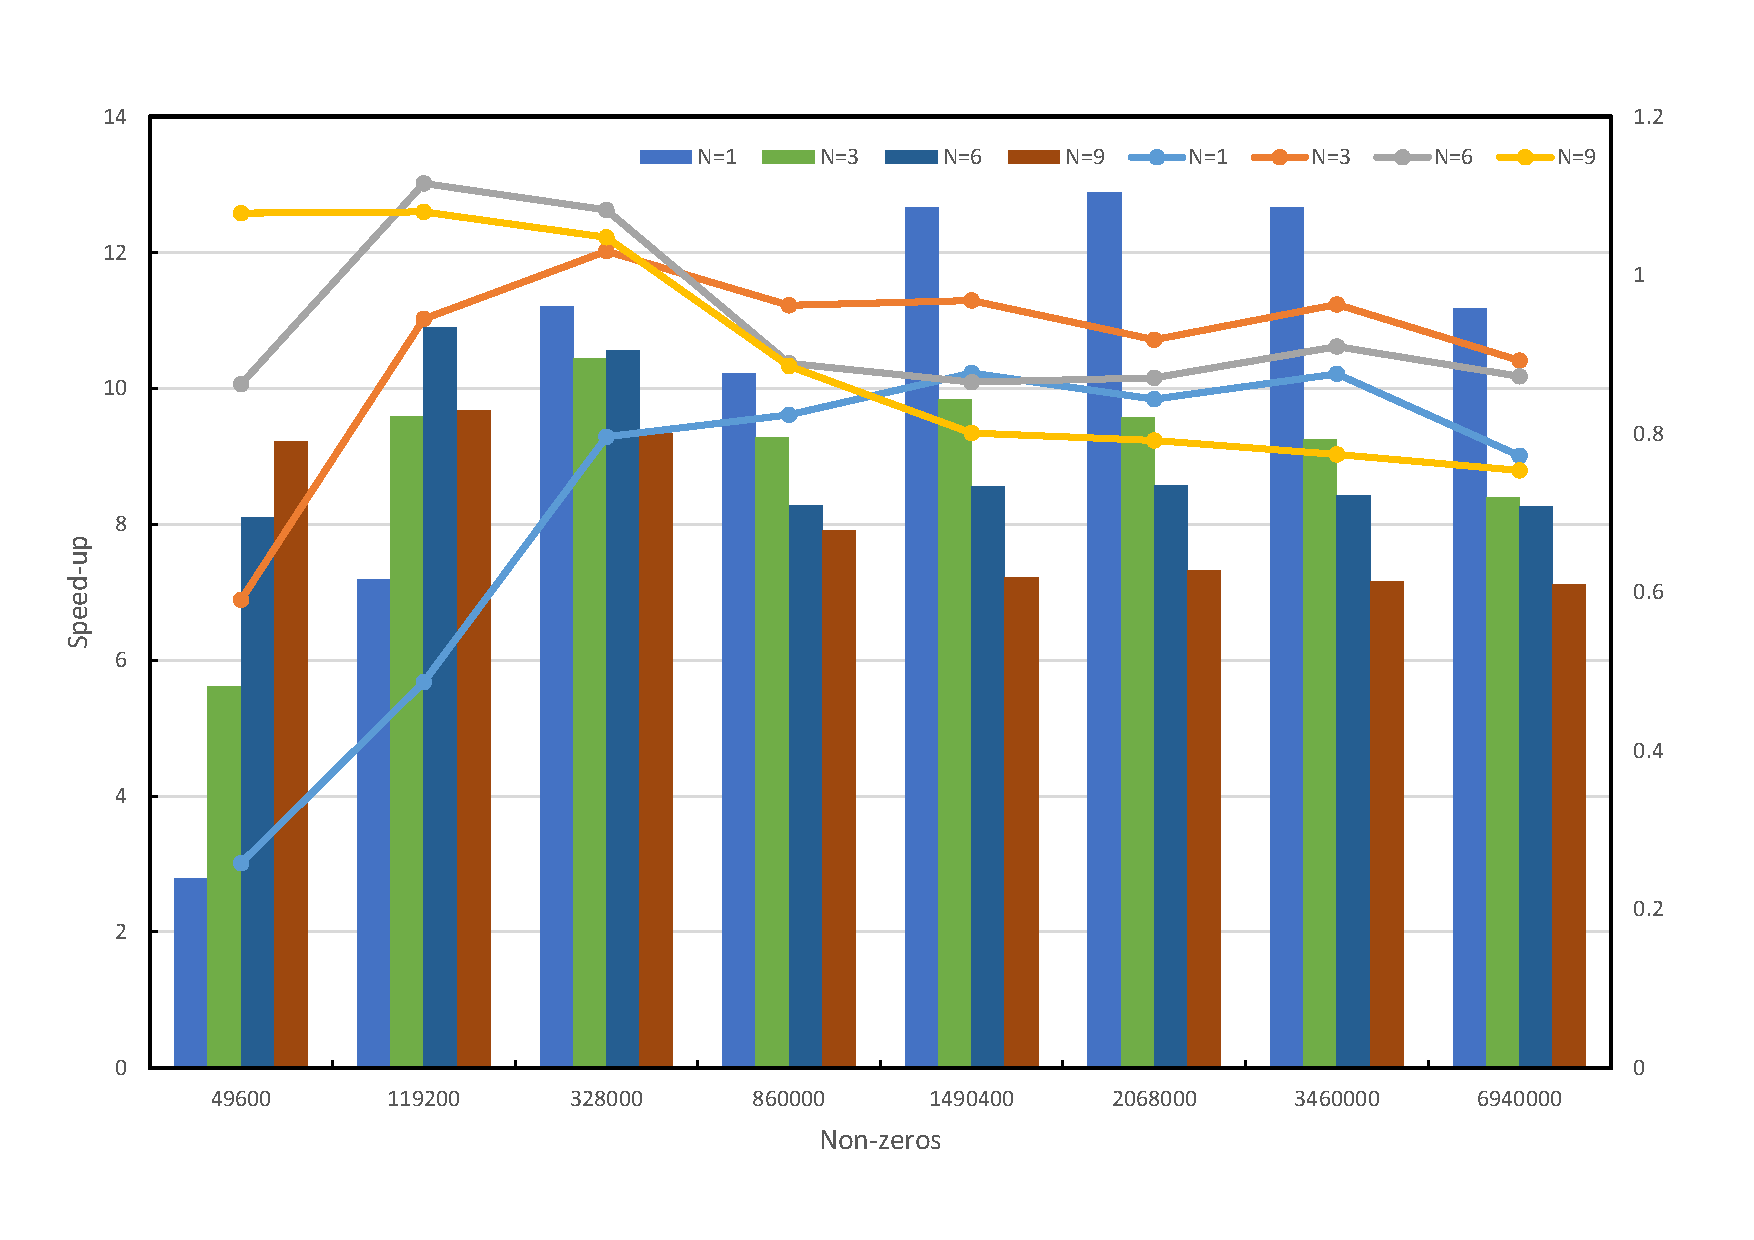
\includegraphics[width=0.47\textwidth]{mlb(ldu).pdf}}
\caption{The speed-up of MLB iterator with LDU format compared to the baseline.}
\label{mlbldu}
\end{figure}
The speed-up of MLB iterator slightly increases with the number of non-zeros and reach its best performance around 2 million entries. The reported speed-up is around 12 when $N=1$ while about 70 percent of performance can be obtained under other circumstance. The reason can be summarized as three factors.

firstly, the AOS storage pattern is not friendly to many-core architectures because of the exist of stride between different components \cite{b10}\cite{b11}. Secondly, the topology of RLC is only determined by the topology of matrix and independent of the data storage pattern to fulfill the compatibility, so the RLC will be performed $N$ times, which equals to number of components. Finally, within the limited LDM space, the number of blocks has a variation of direct proportion with the number of components while the non-zeros assigned to one CPE takes the reverse direction. The increase of proportion of off-diagonal blocks indicates the increase of communication boundary among CPEs, which gives severe pressure to the RLC.

However, we can not conclude from the speed-ups that we can get better performance from SOA storage pattern than AOS for MLB iterator. The speed-ups only reveal the performance of one of the components in SOA while these components are managed in the outer loop serially. An more precise measurement about the performance of SOA and AOS is the Floating-point operations per second (Flops), which is also presented in Fig. \ref{mlbldu}. The Flops of AOS is slightly higher than SOA except for $N=9$ when the matrix size is large enough, and for the smallest matrix the Flops of $N=9$ is the highest. This implies that SOA storage pattern is the better choice for MLB iterator in view of the performance, which can also be demonstrated in Fig. \ref{mlbcsr}.

On the other hand, Fig. \ref{mlbcsr} illustrates the performance of MLB iterator with CSR format.
\begin{figure}[tbp]
\centerline{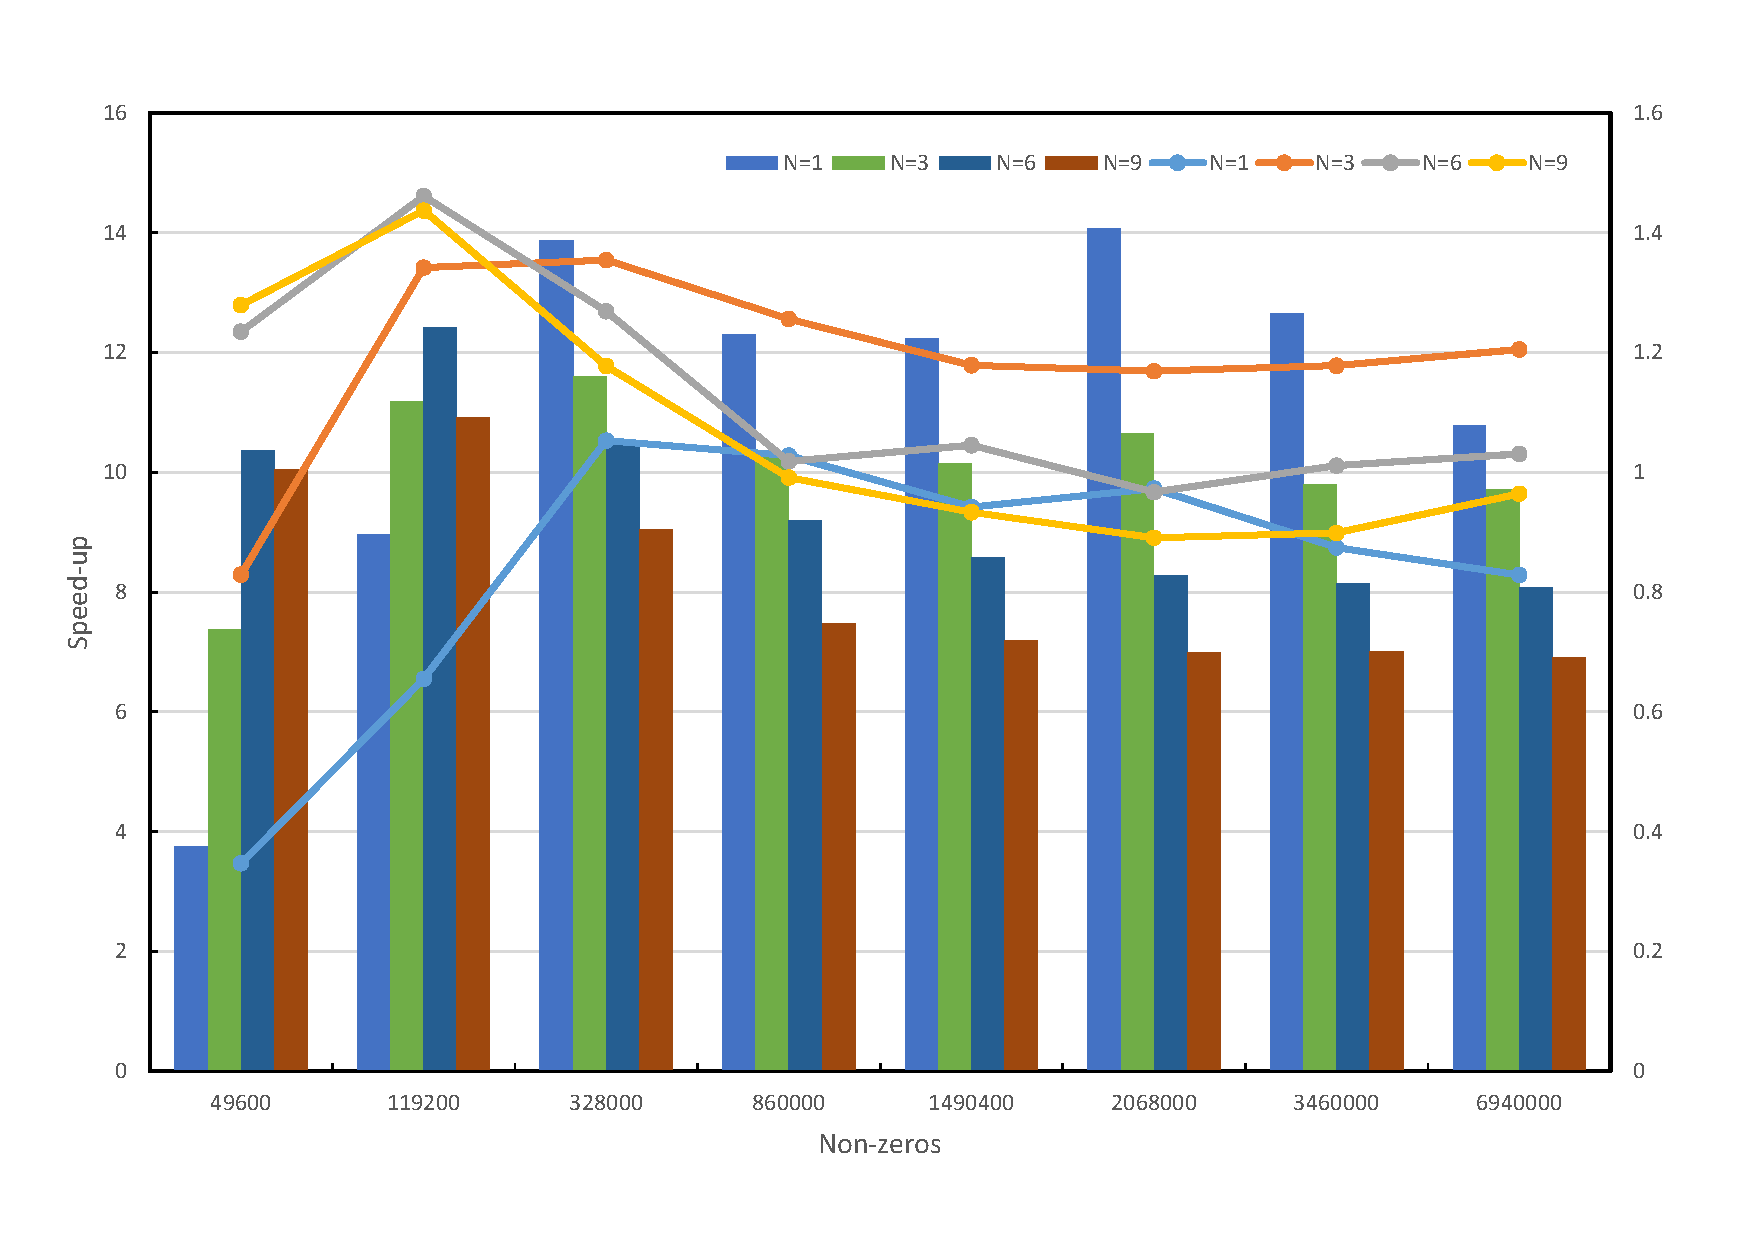
\includegraphics[width=0.47\textwidth]{mlb(csr).pdf}}
\caption{The speed-up of MLB iterator with CSR format compared to the baseline.}
\label{mlbcsr}
\end{figure}
The trend with respect to AOS and SOA is similar to LDU, but it is obvious that we obtain 10~20 percent performance gain from CSR format whether AOS or SOA. The main advantage of CSR format is the absence of write conflicts. For LDU format, RLC will be perform twice to transfer $x$ and $b$, while only $x$ need to be transfer through RLC for CSR format. However, this benefit is at the cost of redundant computations, similar to the "owner-compute" model\cite{b12}, while it is not evident for SpMV because of the existence of lower triangle. In some flux computation of finite volume scheme, the sparse matrix is symmetric structurally and numerically and then the computation of lower triangle is needless. But the cost of redundant computations in CSR format is not so evident for Sunway processor benefiting from its higher ratio of computing capacity and memory bandwidth and then the performance of these two matrix format for one certain problem has to be measured and analyzed dialectically.

\subsection{Results of RSS Iterator}

In this section, we select ten Goodwin matrices from the University of Florida Sparse Matrix Collection. Goodwin is a finite-element matrix in a nonlinear solver, provided by Ralph Goodwin of the University of Illinois at Urbana-Champaign. The performance of RSS iterator with LDU format is presented in Fig. \ref{rssldu}.
\begin{figure}[tbp]
\centerline{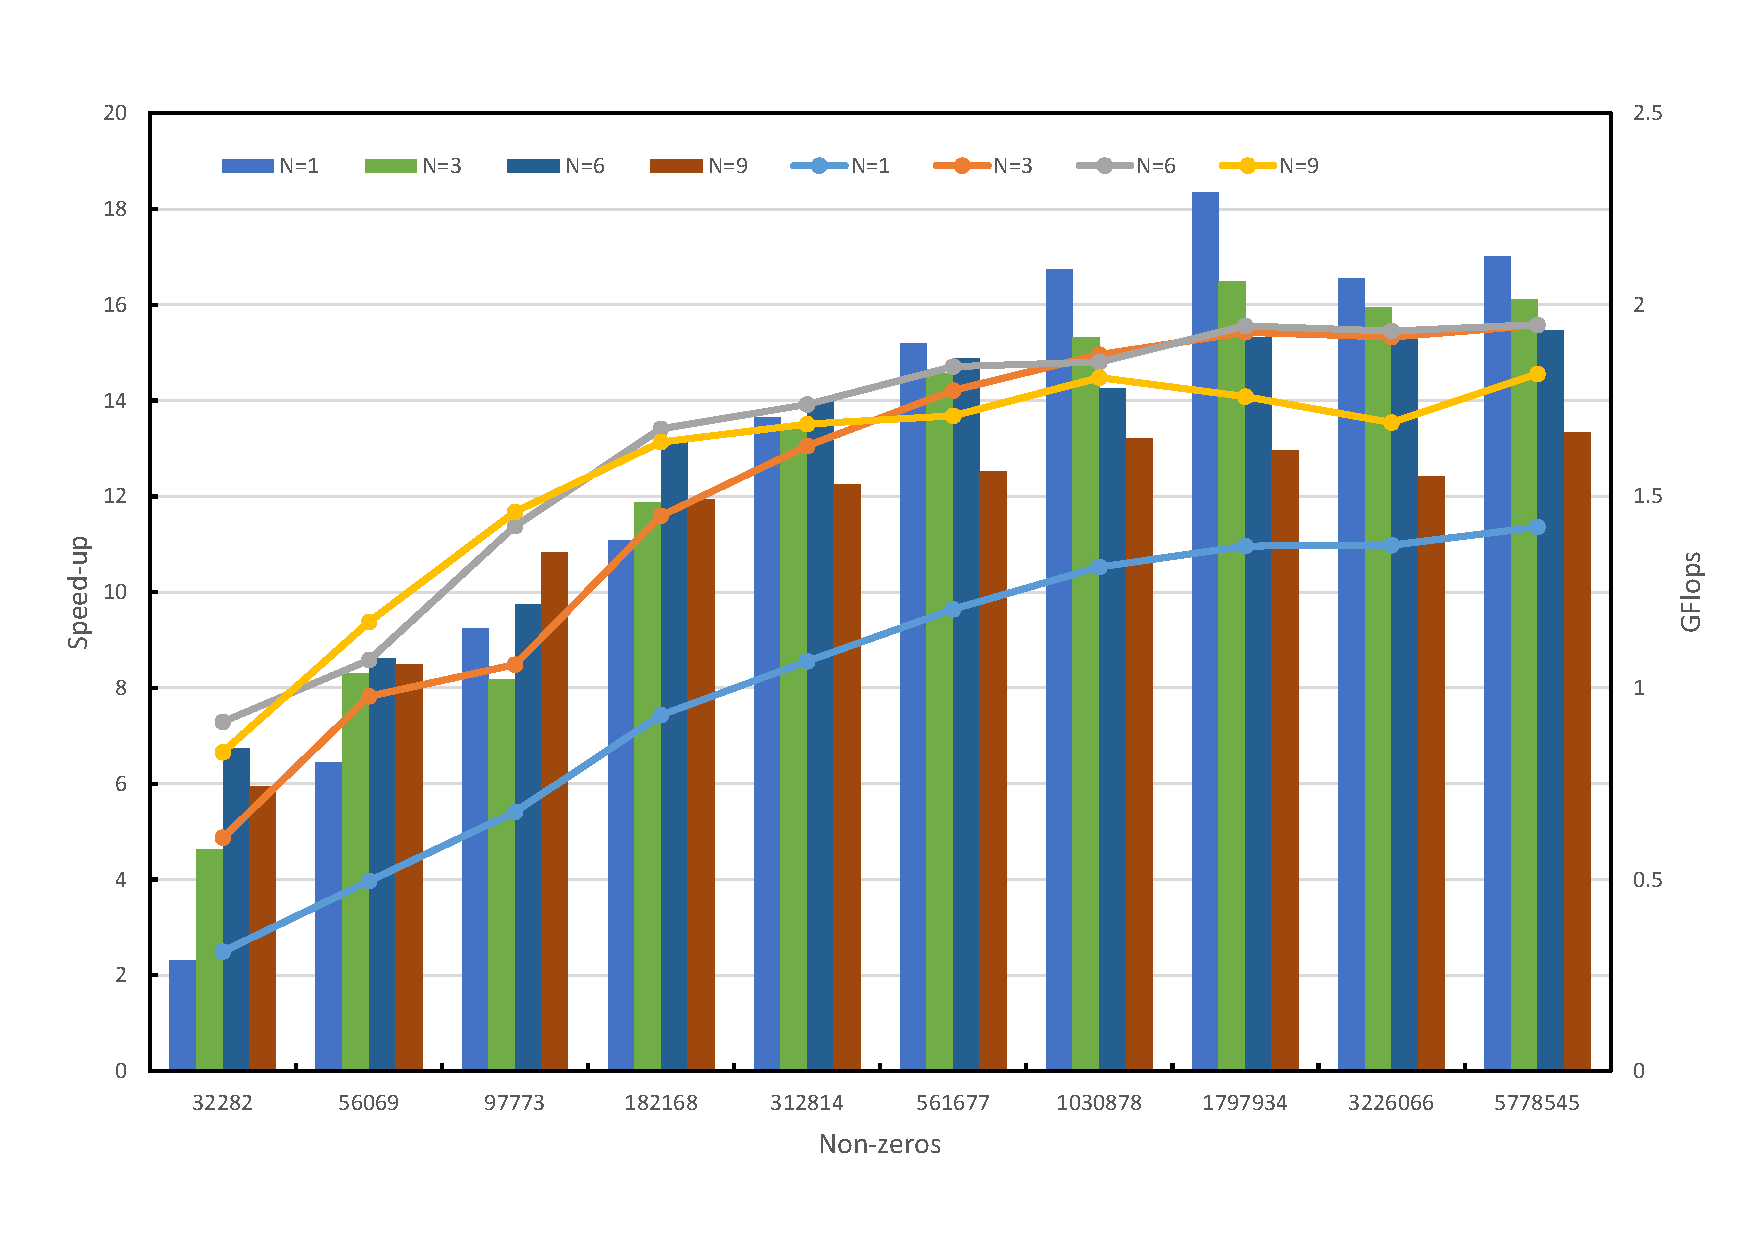
\includegraphics[width=0.47\textwidth]{rss(ldu).pdf}}
\caption{The speed-up of RSS iterator with LDU format compared to the baseline.}
\label{rssldu}
\end{figure}
In general, our implementation achieves 15x speed-up on average compared to the base line and the Flops reach almost 2 GFlops. The obvious gap between AOS and SOA is primarily caused by the write-round-by-round. As mentioned above, the bandwidth of DMA nearly reach its peak performance when the size of continuous memory access blocks is over 1024 Bytes. Hence the length $L$ of column-section is determined by (\ref{colLen}),
\begin{equation}
\label{colLen}
    L=\frac{1024}{sizeof(swFloat)\times N)}
\end{equation}
where $N$ is the number of components in struct.
Compared to the SOA pattern ($N=1$), AOS pattern has shorter column-section, which provides two benefits for DMA: firstly, it reduces the ratio of redundant rows without the bandwidth changed; Moreover, the shorter column-section indicates the less overlap of column-section across the CPEs, which reduces the amount of DMA rounds.

Fig. \ref{rsscsr} illustrates the performance of RSS iterator with CSR format.
\begin{figure}[tbp]
\centerline{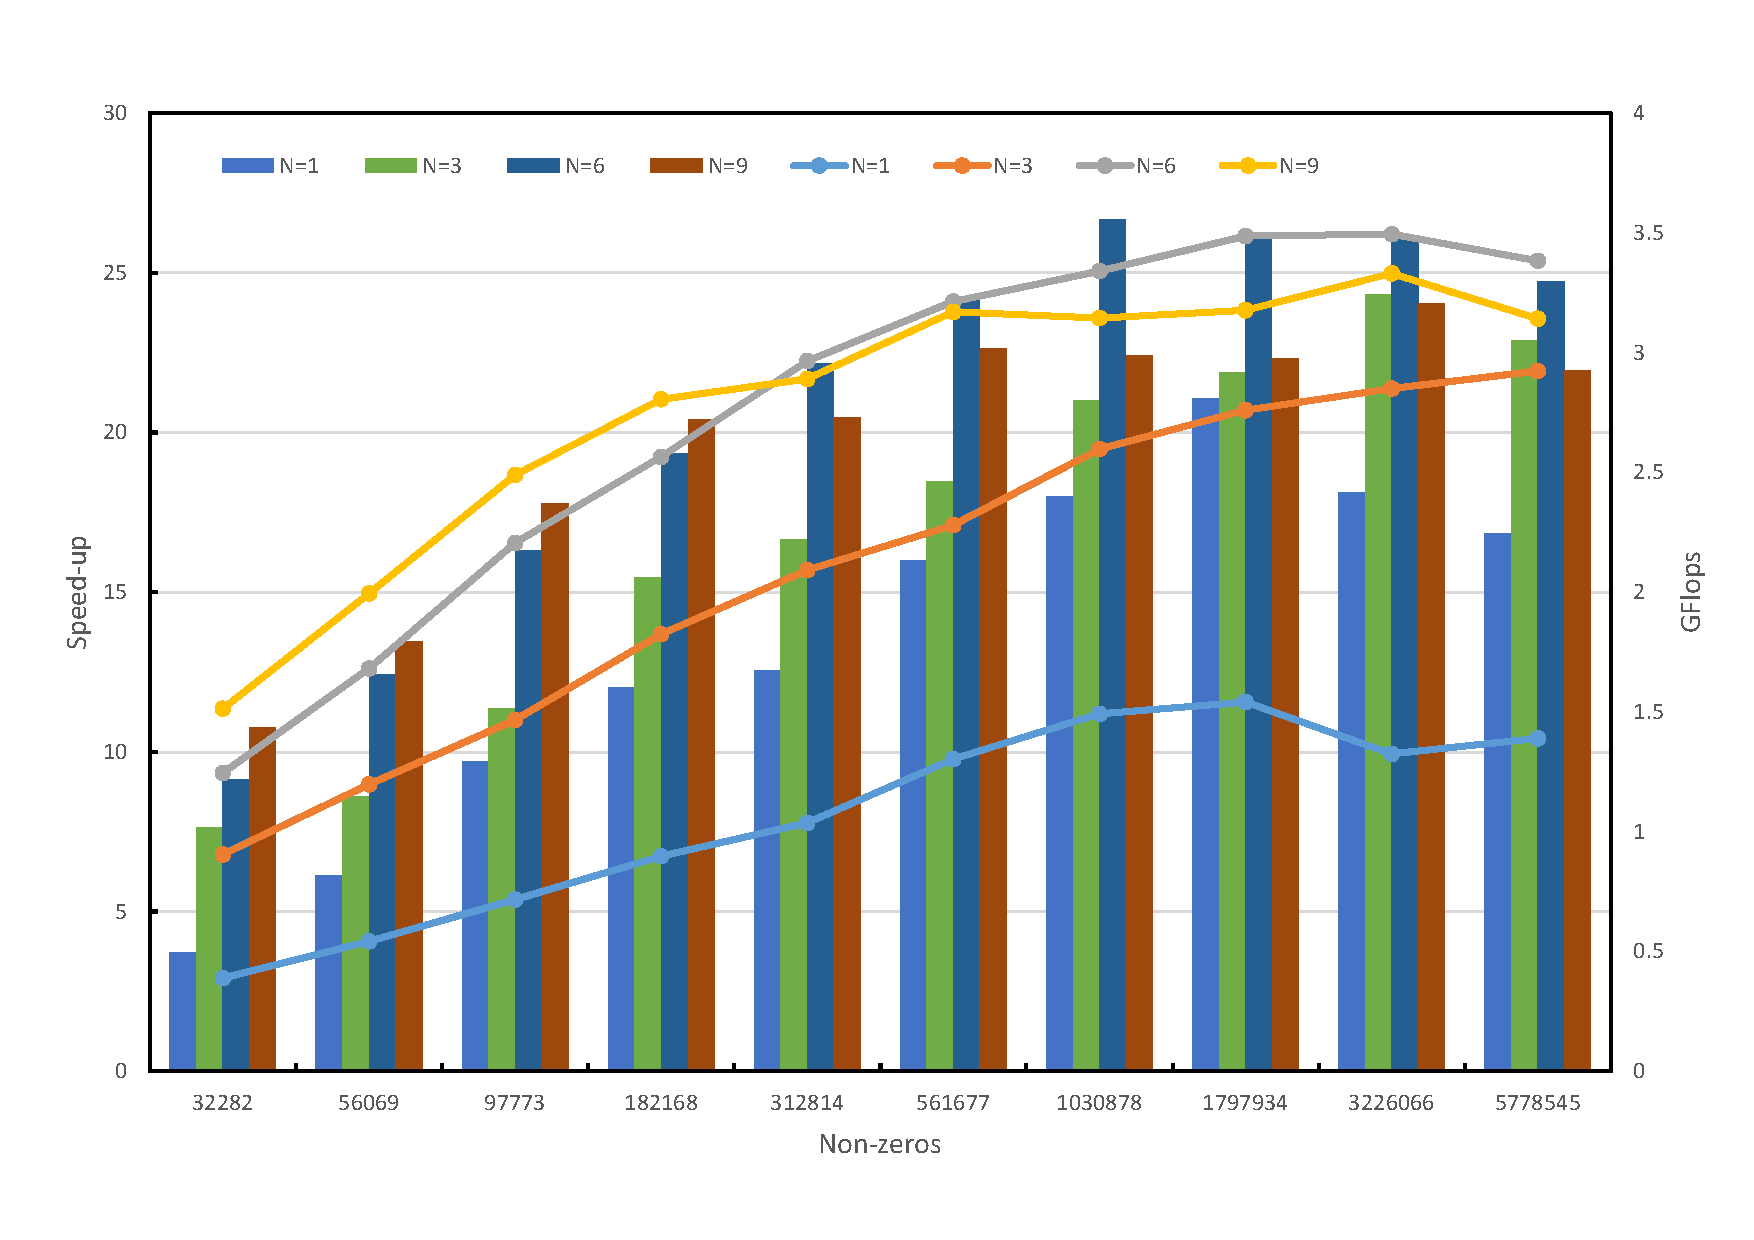
\includegraphics[width=0.47\textwidth]{rss(csr).pdf}}
\caption{The speed-up of RSS iterator with CSR format compared to the baseline.}
\label{rsscsr}
\end{figure}
The highest reported speed-up and Flops reach nearly 27 and 3.5 GFlops respectively and the overall performance of CSR pattern is 1.5x compared to LDU pattern. The obvious difference is caused by write conflict, which has been explained in the last section. Similarly, the redundant computation becomes "meaningful" with the existence of lower triangle in SpMV operator. Therefore, we take the convective flux computation of an unstructured finite-volume solver as example. This solver is an well-tuned in-house cell-centred flow equation solver \cite{b13}\cite{b14}, which can perform RANS, LES and hybrid RANS/LES simulations. The convective flux is discretized with a second-order hybrid upwind/central scheme, which is based on the Roe upwind scheme \cite{b15}. The specifications and results are presented in \ref{umbt_conv}.
% Please add the following required packages to your document preamble:
% \usepackage{multirow}
\begin{table}[]
\caption{performance of convective flux computation with different format}
\begin{tabular}{|c|c|c|c|c|}
\hline
Matrix                        & Format & Time(CPEs) & Speed-up & Flops(G) \\ \hline
\multirow{2}{*}{Goodwin\_071} & LDU    & 25758      & 24.8     & 17.9     \\ \cline{2-5} 
                              & CSR    & 31363      & 35.4     & 29.4     \\ \hline
\end{tabular}
\label{umbt_conv}
\end{table}
Although we obtain higher flops from CSR format, half of them is redundant computation. LDU format has the shorter absolute execution time, which is fundamentally important for flux computation. Therefore, we should switch between these two formats to pursue higher performance in scientific computation, which is convenient in UNAT.

We propose an method to analyze the utilization ratio of Sunway processor with UNAT. The time costed by DMA and operator, $T_{DMA}$ and $T_{ops}$, is thoroughly determined by the problem type and specification of processor, which is non-optimizable for general accelerated framework like UNAT. This part of time can be concluded as follows:
\begin{equation}
\begin{aligned}
    T_{DMA}+T_{ops}&=\frac{S_{DMA}}{BW_{the}}+\frac{N_{ops}}{Flops_{the}} \\
    &=(\frac{BW_{act}}{BW_{the}}+\frac{Flops_{act}}{Flops_{the}})\times T
\end{aligned}
\end{equation}
$S_{DMA}$ is the sum of rows and non-zeros of matrix $A$, vector $x$ and vector $b$ with the components into consideration and $N_{ops}$ is the amount of operations. The theoretical bandwidth $BW_{the}$ and Flops $Flops_{the}$ is easy to obtain from the manual guide of SW26010. The actual bandwidth $BW_{act}$ and Flops $Flops_{act}$ can be obtain from the above results. Here we define $\tau$ as the utilization ratio of Sunway processor:
\begin{equation}
    \tau =\frac{T_{DMA}+T_{ops}}{T}
\end{equation}
The utilization ratio of RSS iterator with CSR format is presented in Fig. \ref{tau}.
\begin{figure}[tbp]
\centerline{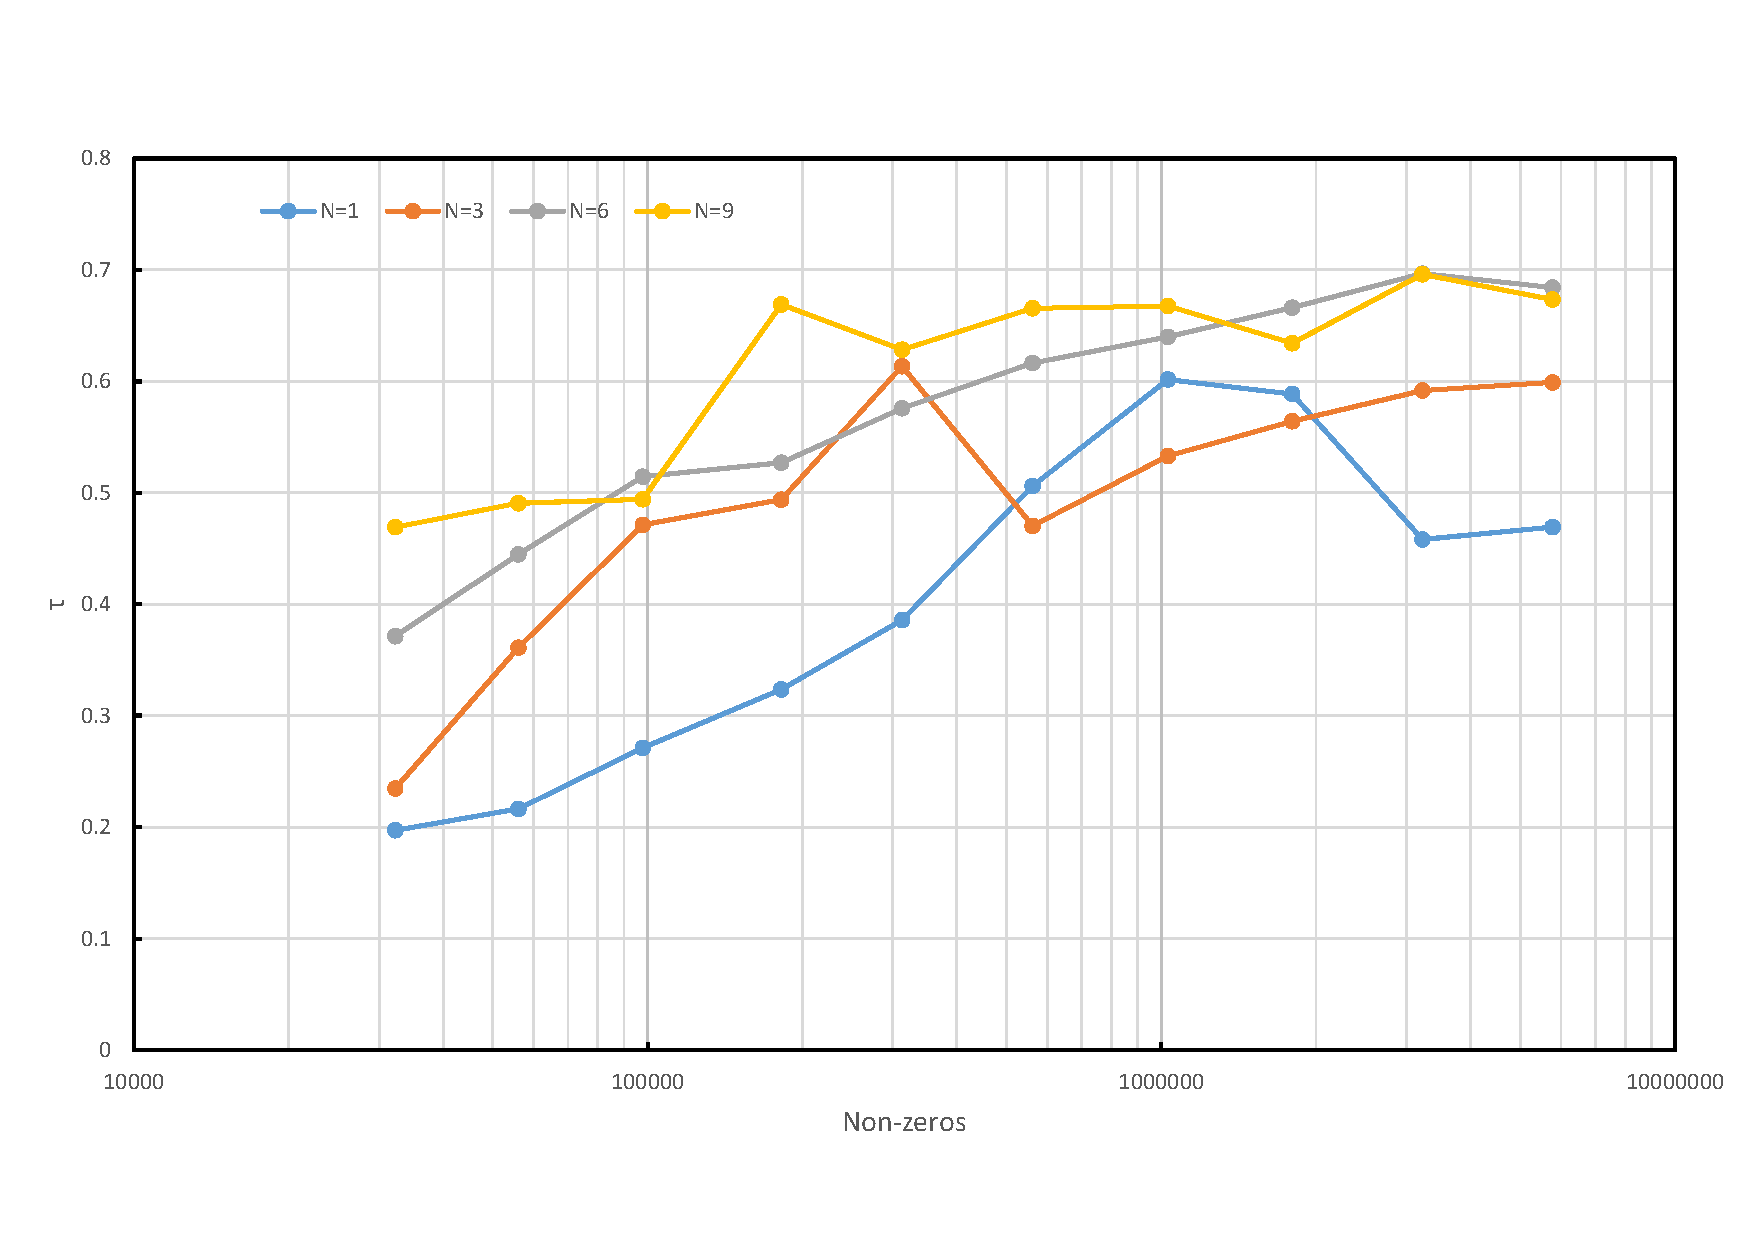
\includegraphics[width=0.47\textwidth]{tau.pdf}}
\caption{The utilization ratio of RSS iterator with CSR format.}
\label{tau}
\end{figure}
The data-sets and configuration are identical to the above experiments. It is clear that UNAT can utilize 60\% performance of Sunway processor on average. Considering its universality and compatibility, the performance of UNAT is acceptable and reasonable.

\section{Conclusion}

\section*{Acknowledgment}

The preferred spelling of the word ``acknowledgment'' in America is without 
an ``e'' after the ``g''. Avoid the stilted expression ``one of us (R. B. 
G.) thanks $\ldots$''. Instead, try ``R. B. G. thanks$\ldots$''. Put sponsor 
acknowledgments in the unnumbered footnote on the first page.

\section*{References}

Please number citations consecutively within brackets \cite{b1}. The 
sentence punctuation follows the bracket \cite{b2}. Refer simply to the reference 
number, as in \cite{b3}---do not use ``Ref. \cite{b3}'' or ``reference \cite{b3}'' except at 
the beginning of a sentence: ``Reference \cite{b3} was the first $\ldots$''

Number footnotes separately in superscripts. Place the actual footnote at 
the bottom of the column in which it was cited. Do not put footnotes in the 
abstract or reference list. Use letters for table footnotes.

Unless there are six authors or more give all authors' names; do not use 
``et al.''. Papers that have not been published, even if they have been 
submitted for publication, should be cited as ``unpublished'' \cite{b4}. Papers 
that have been accepted for publication should be cited as ``in press'' \cite{b5}. 
Capitalize only the first word in a paper title, except for proper nouns and 
element symbols.

For papers published in translation journals, please give the English 
citation first, followed by the original foreign-language citation \cite{b6}.

\begin{thebibliography}{00}
\bibitem{b1} G. Eason, B. Noble, and I. N. Sneddon, ``On certain integrals of Lipschitz-Hankel type involving products of Bessel functions,'' Phil. Trans. Roy. Soc. London, vol. A247, pp. 529--551, April 1955.
\bibitem{b2} J. Clerk Maxwell, A Treatise on Electricity and Magnetism, 3rd ed., vol. 2. Oxford: Clarendon, 1892, pp.68--73.
\bibitem{b3} I. S. Jacobs and C. P. Bean, ``Fine particles, thin films and exchange anisotropy,'' in Magnetism, vol. III, G. T. Rado and H. Suhl, Eds. New York: Academic, 1963, pp. 271--350.
\bibitem{b4} K. Elissa, ``Title of paper if known,'' unpublished.
\bibitem{b5} R. Nicole, ``Title of paper with only first word capitalized,'' J. Name Stand. Abbrev., in press.
\bibitem{b6} Y. Yorozu, M. Hirano, K. Oka, and Y. Tagawa, ``Electron spectroscopy studies on magneto-optical media and plastic substrate interface,'' IEEE Transl. J. Magn. Japan, vol. 2, pp. 740--741, August 1987 [Digests 9th Annual Conf. Magnetics Japan, p. 301, 1982].
\bibitem{b7} M. Young, The Technical Writer's Handbook. Mill Valley, CA: University Science, 1989.

\bibitem{b8} Liu, C., Xie, B., Liu, X., Xue, W., Yang, H., and Liu, X. (2018, June). Towards efficient spmv on sunway manycore architectures. In Proceedings of the 2018 International Conference on Supercomputing (pp. 363-373). ACM.
\bibitem{b9} Davis, T. A., and Hu, Y. (2011). The University of Florida sparse matrix collection. ACM Transactions on Mathematical Software (TOMS), 38(1), 1.
\bibitem{b10} Cook, S. (2012). CUDA programming: a developer's guide to parallel computing with GPUs. Newnes.
\bibitem{b11} Liu, H., Su, X., and Yuan, X. (2018). Accelerating unstructured large eddy simulation solver with GPU. Engineering Computations, 35(5), 2025-2049.
\bibitem{b12} Mudalige, G. R., Giles, M. B., Reguly, I., Bertolli, C., and Kelly, P. H. J. (2012, May). Op2: An active library framework for solving unstructured mesh-based applications on multi-core and many-core architectures. In 2012 Innovative Parallel Computing (InPar) (pp. 1-12). IEEE.
\bibitem{b13} Yuan, X., and Daiguji, H. (2001). A specially combined lower–upper factored implicit scheme for three-dimensional compressible Navier–Stokes equations. Computers and fluids, 30(3), 339-363.
\bibitem{b14} Su, X. (2015). Accurate and robust adaptive mesh refinement for aerodynamic simulation with multi‐block structured curvilinear mesh. International Journal for Numerical Methods in Fluids, 77(12), 747-766.
\bibitem{b15} Roe, P. L. (1981). Approximate Riemann solvers, parameter vectors, and difference schemes. Journal of computational physics, 43(2), 357-372.
\bibitem{b16} Fang, J., Fu, H., Zhao, W., Chen, B., Zheng, W., and Yang, G. (2017, May). swdnn: A library for accelerating deep learning applications on sunway taihulight. In 2017 IEEE International Parallel and Distributed Processing Symposium (IPDPS) (pp. 615-624). IEEE.

\end{thebibliography}
\vspace{12pt}
\color{red}
IEEE conference templates contain guidance text for composing and formatting conference papers. Please ensure that all template text is removed from your conference paper prior to submission to the conference. Failure to remove the template text from your paper may result in your paper not being published.

\end{document}
